\subsection{Annichilazione in 3 fotoni}

%teoria
\subsubsection{Stime teoriche}
Lo scattering $e^+e^-$ può produrre uno stato finale con 3 fotoni: il rapporto teorico dei branching ratio tra questo processo e la più comune annichilazione in 2 fotoni è $\sim 1/378$\cite{3gamma}. La distribuzione angolare attesa per i 3 fotoni prodotti è rappresentata in \autoref{fig:3gamma_angular_distr}. Se il decadimento avviene a riposo nel sistema del laboratorio\footnote{ipotesi ragionevole nel nostro caso e suffragata dall'osservazione in \autoref{positron_momentum}} i fotoni sono vincolati ad essere emessi su un piano: quindi fissata la direzione di 2 fotoni, il terzo è vincolato ad essere emesso su un arco di circonferenza i cui limiti sono fissati dalla conservazione dell'energia. A causa di questi vincoli e poiché i nostri spettrometri rivelano solo in un certo angolo solido, il rate dei conteggi per questo tipo di segnale sarà inversamente proporzionale a $d^5$ dove $d$ è la distanza dei rivelatori (nel caso semplice in cui sono alla stessa distanza).
Come visibile in \autoref{fig:3gamma_angular_distr} la probabilità relativa di emissione varia poco negli angoli permessi (variazione massima del $\sim 25\%$) e per i nostri scopi è ragionevolmente uniforme per angoli intorno a $\alpha\simeq \SI{120}{\degree}$ e $\beta\simeq\SI{120}{\degree}$.
Le energie dei 3 fotoni al variare degli angoli sono facilmente ricavabili dalla conservazione del quadrimpulso:
\begin{align*}
\label{eq:3gamma_energy}
E_3 &= \frac{2 m_e}{\frac{\sin\beta \;+\;(1+\cos\alpha)}{\sin\alpha}+\cos\beta+1}\\
E_2 &= E_3 \cdot \frac{\sin\beta}{\sin\alpha}\\
E_1 &= 2m_e - E_2 - E_3\\
\end{align*}
dove $\alpha$ e $\beta$ sono rispettivamente gli i supplementari degli angoli tra il fotone 1 e i fotoni 2 e 3.

\begin{figure}[h]
	\centering
	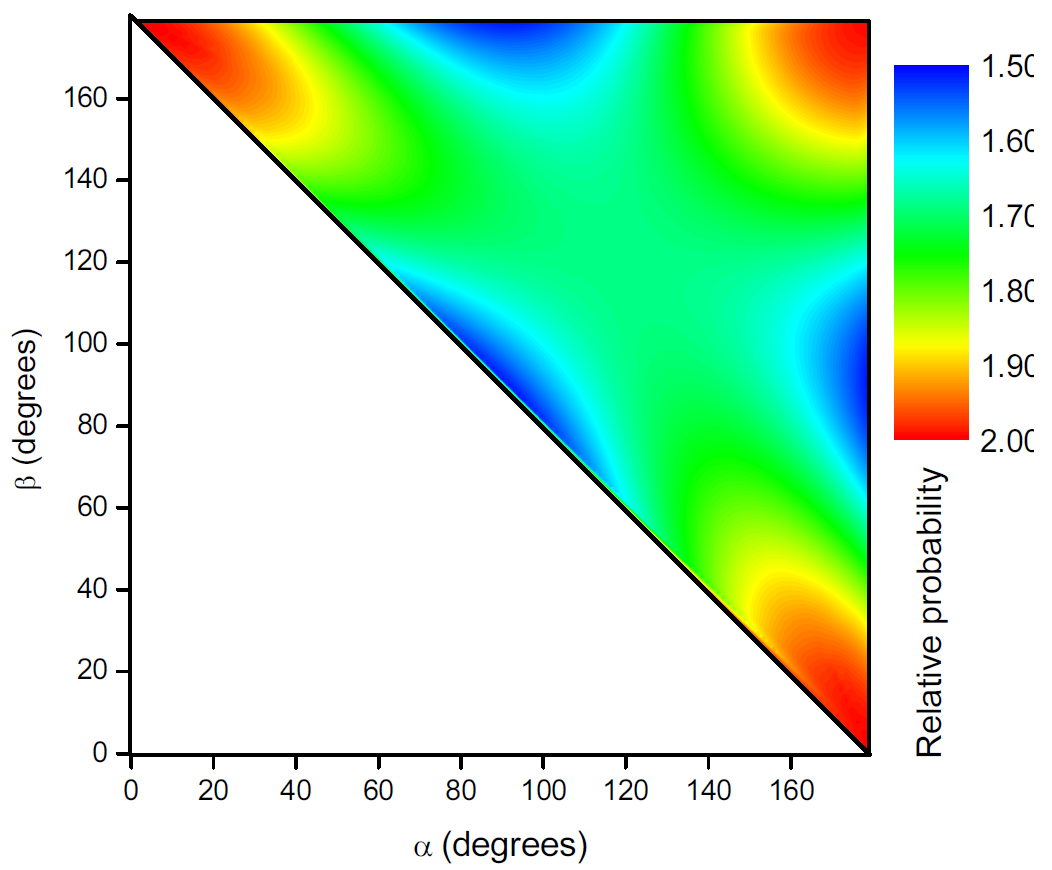
\includegraphics[width=20em]{immagini/3gamma_distribution}
	\caption{\label{fig:3gamma_angular_distr}Probabilità di una data distribuzione angolare per l'annichilazione a 3 fotoni. $\alpha$ e $\beta$ sono rispettivamente gli angoli tra il fotone 1 e i fotoni 2 e 3. La scala della probabilità e arbitraria.}
\end{figure}
%progettazione dell'esperimento

Una stima dell'ordine di grandezza del numero di eventi di segnale attesi è ottenibile a partire dalla formula:
\begin{equation}
\label{eq:stima_3gamma}
N_{3\gamma} \simeq T \cdot R_{\beta^+} \cdot \frac{\text{BR}(3\gamma)}{\text{BR}(2\gamma)} \cdot \text{Acc} \cdot \text{Eff} \cdot R_{p2t} \cdot 3!
\end{equation}
Dove:
\begin{itemize}
	\item $T$ è il tempo di presa dati, realisticamente dell'ordine di $\SI{10}{h}$;
	\item $R_{\beta^+}$ è il rate di emissione di positroni della nostra sorgente principale, dell'ordine di $\SI{500}{kBq}$;
	\item $\frac{\text{BR}(3\gamma)}{\text{BR}(2\gamma)}$ è il rapporto dei branching ratio dei due processi ed è atteso essere $1/378$;
	\item Acc è l'accettanza combinata dei tre rivelatori che possiamo stimare in $\sim \frac{r^5}{2^7 d^5}$\footnote{questa è solo una stima dell'integrale dello spazio delle fasi a 3 corpi} dove $r$ è il raggio dei rivelatori ($1''$) e che ad una distanza di $\SI{20}{cm}$ dà un'accettanza del $\sim\SI{2e-7}{}$;
	\item Eff è l'efficienza intrinseca combinata dei tre spettrometri che per rivelatori di NaI $2''\times2''$ è nota \cite{knoll} e all'energia di $\sim \SI{300}{keV}$ vale circa $(90\%)^3 \simeq  70\%$;
	\item $R_{p2t}$ è il rapporto tra gli eventi nel picco fotoelettrico e il totale, anche questo noto \cite{knoll} e alla stessa energia vale circa $(60\%)^3 \simeq 20\%$;
	\item il fattore $3!$ serve a tener conto della molteplicità.
\end{itemize}
\subsubsection{Rumore}
Il risultato della stima è circa 10 eventi. A questo punto è necessario stimare/misurare il rumore.
Il rate di coincidenze a 3 in alcune configurazioni provate è in ogni caso molto maggiore del segnale atteso è quindi necessario ottimizzare il rapporto segnale/rumore per rendere visibile il segnale.
Le coincidenze casuali sono depresse dal fatto che si tratta di una coincidenza a tre e la sorgente principale di rumore è la sorgente stessa: 
anche se la sorgente non si trova sulla congiungente di nessuna coppia di rivelatori, rendendo di fatto impossibile rilevare direttamente la coppia di fotoni back-to-back prodotti nell'annichilazione, è comunque possibile che la coincidenza a tre scatti e possa esserci un evento indistinguibile dal segnale:
\begin{itemize}
	\item il $\gamma_{\text{Ne}}$\footnote{Nel seguito useremo la notazione $\gamma_{\text{Ne}}$ per indicare i fotoni prodotti dal decadimento del $^{22}\text{Ne}$ e con $\gamma_{\beta}$ quelli prodotti dall'annichilazione in due fotoni.} passa per il rilevatore 1 e ci interagisce facendo scattering Compton;
	\item un $\gamma_{\beta}$ fa scattering Compton nel rivelatore 2;
	\item l'altro $\gamma_{\beta}$ fa scattering Compton o Rayleigh nel materiale che circonda la sorgente (la scatola di metallo che la contiene, il piombo e le pareti in piombo nelle vicinanze) venendo deviata e successivamente interagisce nel rivelatore 3.
\end{itemize}
Un evento del genere farebbe scattare la coincidenza e al variare degli angoli di scattering potrebbe portare ad un evento simile al segnale per energia rilasciata dei rivelatori. Un'altro possibile evento di rumore è quello in cui:
\begin{itemize}
	\item un $\gamma_{\beta}$ fa scattering Compton nel rivelatore 1 e l'altro è perso;
	\item il $\gamma_{\text{Ne}}$ fa scattering Compton nel rivelatore 2 e il fotone uscente dal processo di scattering interagisce con il rivelatore 3.
\end{itemize}
Chiaramente molti altri possibili rimbalzi sono possibili e possono risultare simili al segnale, ma ogni rimbalzo riduce sostanzialmente la probabilità dell'evento: un ``rimbalzo'' dal rivelatore 2 al 3 come nell'esempio precedente è soppresso dal fatto che il back-scattering Compton è sfavorito e dall'accettanza del rivelatore 3 visto dal 2 che, in prima approssimazione, va come $\frac{1}{(2d)^2}$.
Un metodo per misurare il rumore dovuto alla sorgente, eliminando solo il segnale dell'annichilazione in $3\gamma$, è quello di sollevare/abbassare la sorgente in modo tale che nessun piano possa passare per la sorgente e i tre rivelatori: questo eliminerà il segnale fisico lasciando ragionevolmente immutata la forma del rumore.
\subsubsection{Realizzazione della misura}
Si sono adottati alcuni accorgimenti per migliorare il rapporto segnale rumore:
\begin{itemize}
	\item per aumentare il segnale mettiamo gli scintillatori il più vicino possibile alla sorgente: il segnale cresce con l'inverso di $d^5$ quindi passando da $\SI{20}{cm}$ a $\SI{10}{cm}$ si guadagna un fattore 32;
	\item aspettandoci che i rimbalzi tra un rivelatore e l'altro possano rappresentare una parte rilevante del rumore interponiamo dei blocchi di piombo tra un rivelatore e l'altro, abbastanza spessi da fermare la maggior parte dei fotoni (la lunghezza di interazione per energie nel range $\SI{300/500}{keV}$ è $\sim \SI{0.5}{cm}$ e si sono usati blocchi da $\sim \SI{4}{cm}$);
	\item dopo aver osservato la distribuzione tipica del rumore decidiamo gli angoli a cui effettuare la misura di segnale in modo che l'energia dello stesso sia nella zona con meno rumore possibile: 
\end{itemize}

La misura finale è stata presa nelle condizioni schematizzate in \autoref{fig:schema_3gamma}\marginpar{fare figura} e riproposta nella foto in \autoref{fig:foto_3gamma}, dove sono chiari i vincoli imposti dall'apparato: i PMT1, 2 e 3 distano rispettivamente $\SI{10.4(1)}{cm}$, $\SI{9.4(1)}{cm}$ e $\SI{11.0(1)}{cm}$  dalla sorgente e $\alpha \simeq \SI{59(1)}{\degree}$ e $\beta \simeq \SI{43(1)}{\degree}$. Il picco delle energie attese dei tre fotoni sono $E_1= \SI{397}{keV}$, $E_2 =\SI{277}{keV}$, $E_3=\SI{347}{keV}$.
 \begin{figure}[h]
	\centering
	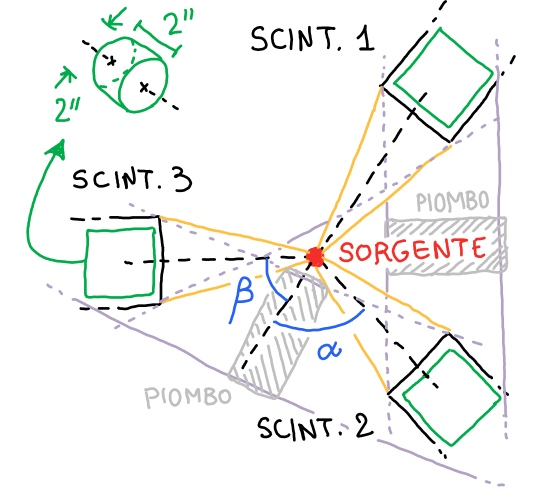
\includegraphics[width=20em]{immagini/schema3gamma}
	\caption{\label{fig:3gamma_signal} Schema dell'apparato utilizzato per la misura del rate di annichilazione in tre fotoni.}
	\label{fig:foto_3gamma}
\end{figure}
Sono state realizzate due prese dati di segnale e una di rumore: sono state svolte quando il laboratorio è chiuso e la risposta dei rivelatori è stabile, con lo stesso obiettivo la parte iniziale e finale della presa dati è stata tagliata: il risultato sono due misure di segnale da $\SI{9.7}{h}$ e $\SI{15.3}{h}$ e una di rumore da $\SI{11.1}{h}$.
 \begin{figure}[h]
	\centering
	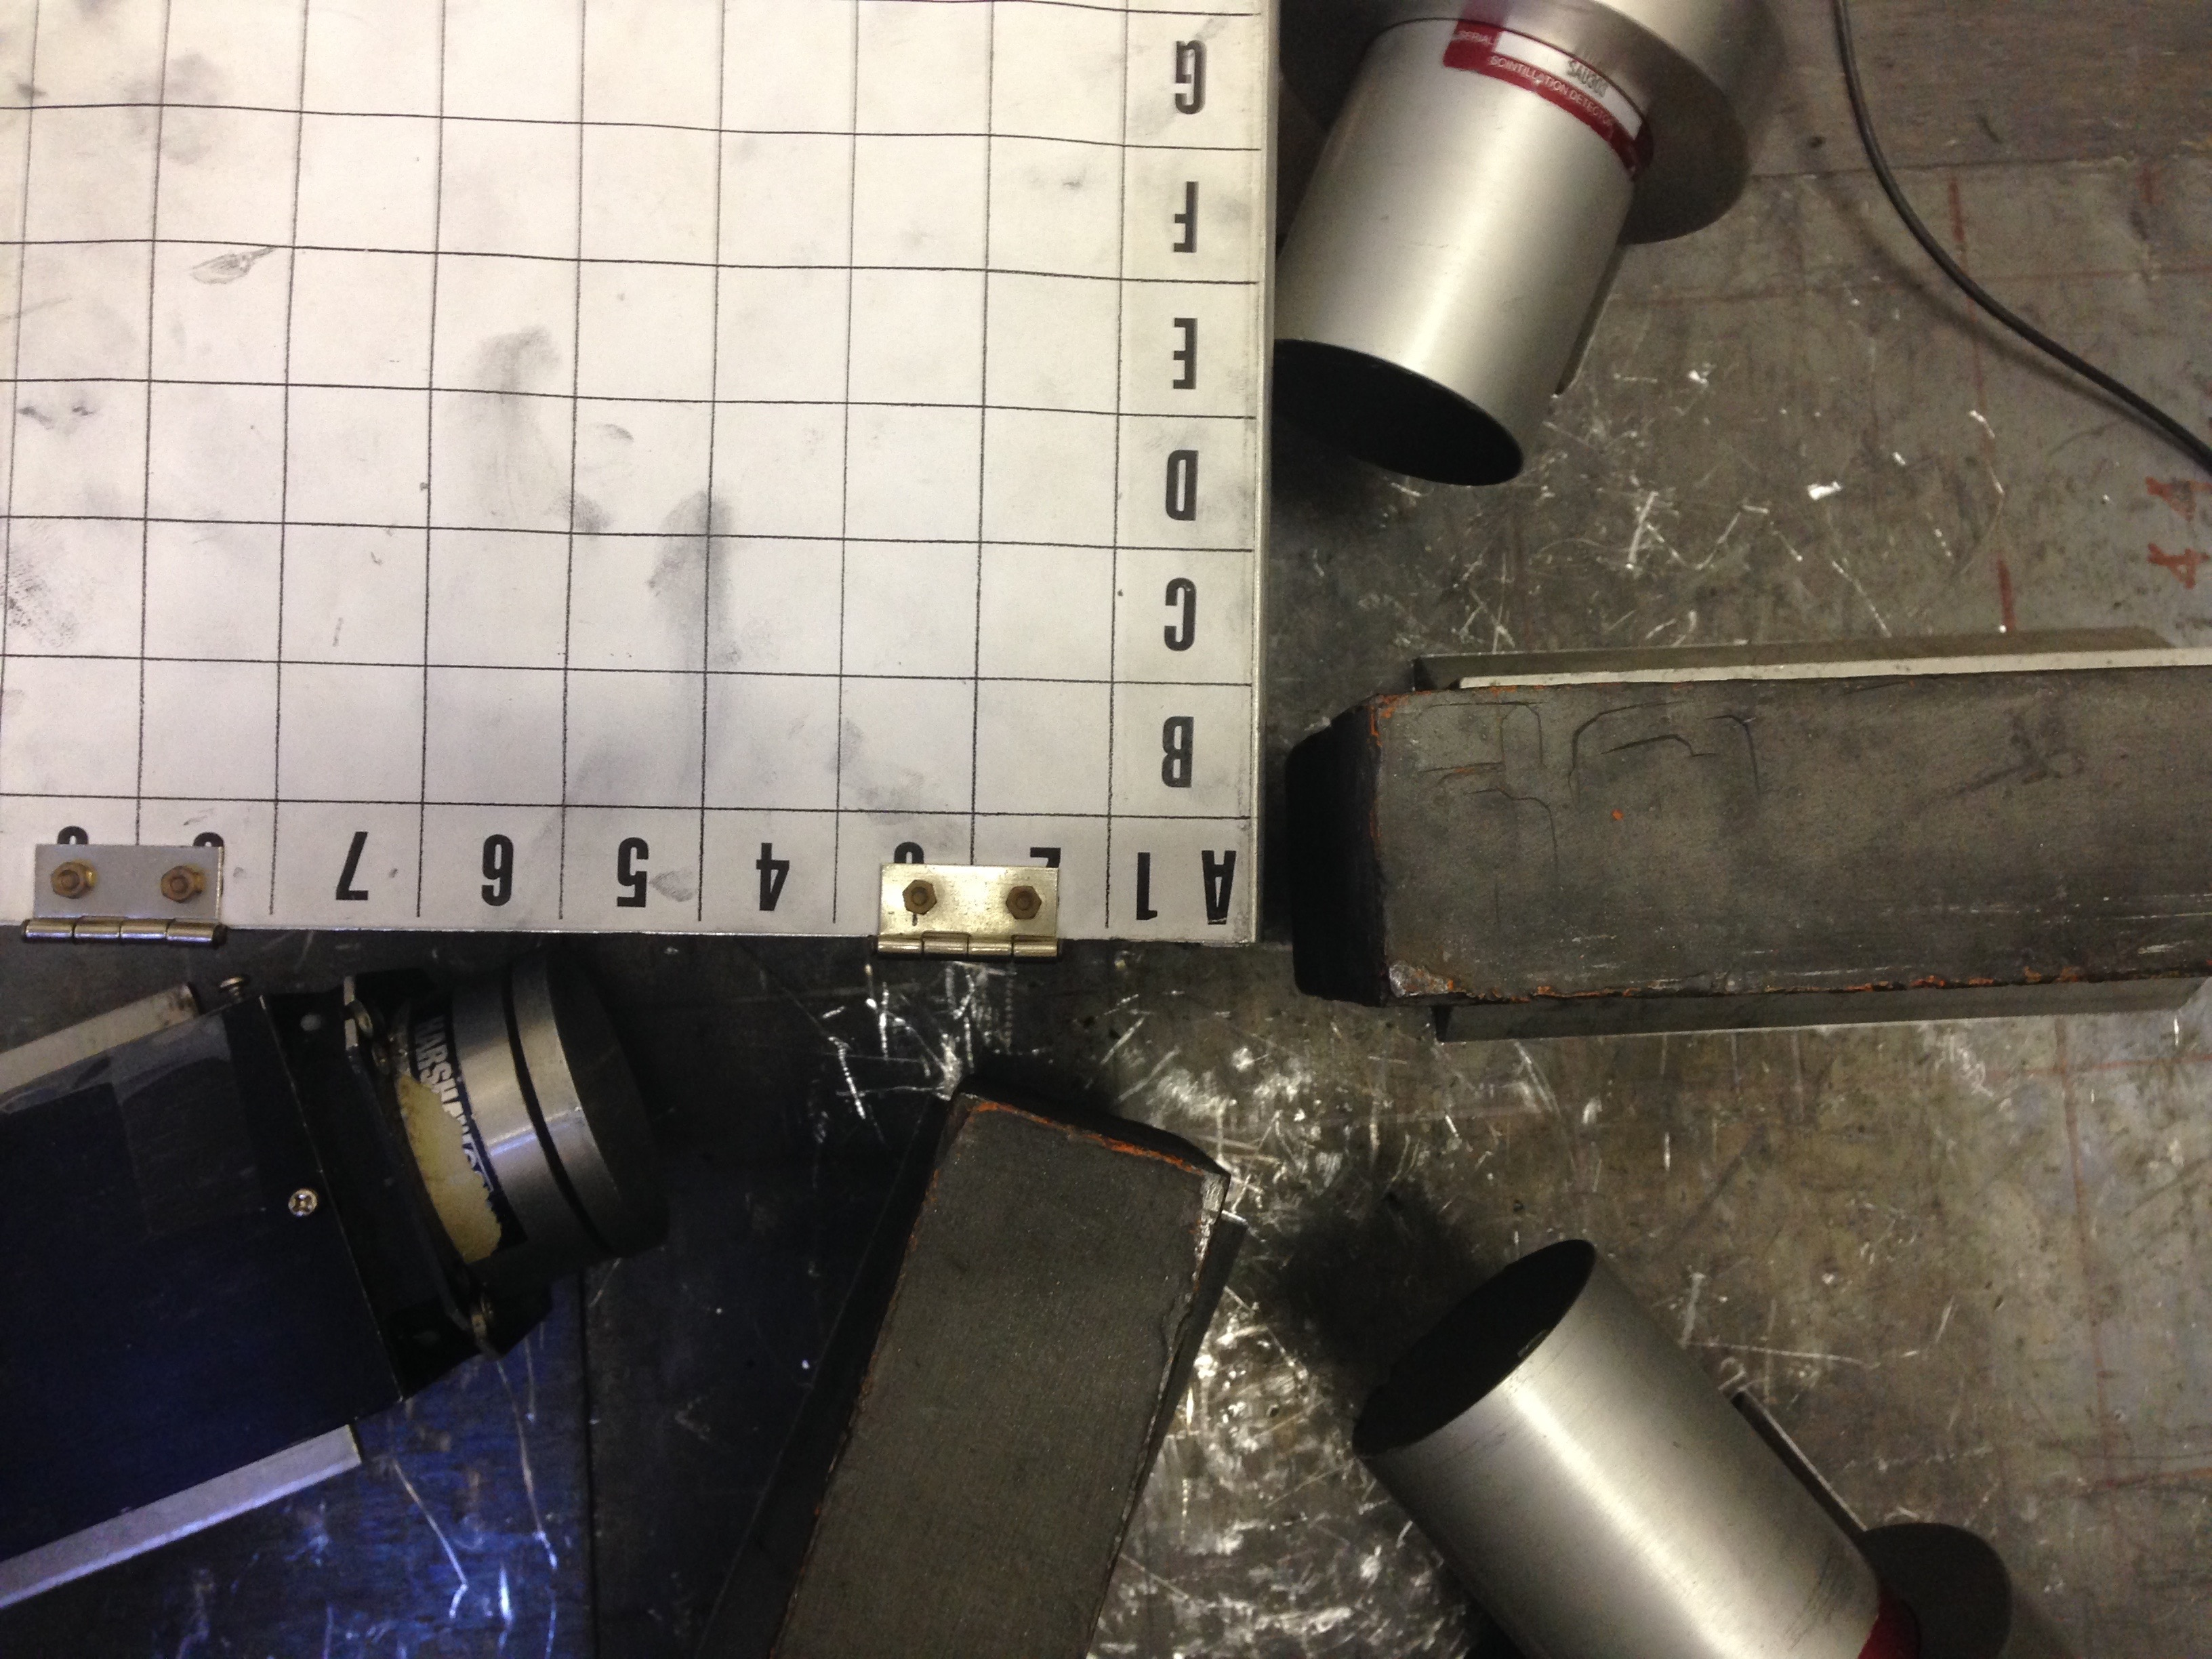
\includegraphics[width=20em]{immagini/3gamma_foto}
	\caption{\label{fig:3gamma_signal} L'apparato utilizzato per la misura del rate di annichilazione in tre fotoni, la sorgente si trova in A1.}
	\label{fig:foto_3gamma}
\end{figure}

\subsubsection{Analisi}
Durante la presa dati sono state misurate e salvate le sole coincidenze a 3. Le energie dei tre rivelatori sono state calibrate per ogni presa dati a partire dai dati stessi, fittando il picco di annichilazione e quello del $^{22}\text{Ne}$ ben visibili nel rumore. I PMT1 e 2 sono stati calibrati con un modello lineare, mentre per il PMT3, notevolmente meno lineare degli altri, si è deciso di usare una parabola passante per 0. Questa scelta è motivata dal fatto che, avendo solo due punti, un'altro vincolo è necessario e non si può fare affidamento sui precedenti fit di risposta parabolica del PMT3 poiché questo si scalibra molto nel tempo e ci interessa la risposta a energie lontane da quelle delle precenti calibrazioni (inferiori al picco di annichilazione); questa scelta può poi essere verificata a posteriori controllando che il segnale sia alla giusta energia su quel canale.

Per stimare l'entità del segnale osservato si è proceduto in due modi.
\paragraph{Stima diretta del rumore}
Determiniamo l'energia a cui ci attendiamo di osservare il segnale e stimiamo la larghezza del picco 3D: l'allargamento è sostanzialmente dovuto a 2 processi:
\begin{itemize}
	\item i fotoni in arrivo non sono monocromatici a causa della dimensione fisica degli scintillatori e gli angoli $\alpha$ e $\beta$ possono variare in un certo range e conseguentemente le energie si troveranno in range massimo:  $E_1 \in [341,437]\si{keV}$, $E_2 \in [246,343]\si{keV}$ e $E_3 \in [337,394]\si{keV}$; si tratta di un range massimo, la forma della distribuzione dipenderà sopratutto dall'efficienza dei PMT che a queste distanze cala lentamente sui bordi;
	\item la risoluzione dello strumento che a queste energie può essere stimata dalla formula (vedi \cite{6}):
	$\sigma_E(E) = a \cdot E \cdot \frac{2.27 + 7.28 \cdot E ^ {-0.29} - 2.41 \cdot E ^ {0.21}} {235}$ e che all'energie di interesse vale circa $\SI{60}{keV}$
\end{itemize}
Si è deciso quindi di selezionare gli eventi in una scatola 3D che contenga la quasi totalità del segnale, in modo da non preoccuparci di dover stimare l'efficienza di questa selezione, complicata da simulare. 
I limiti scelti per la selezione del segnale sono stati: $E_1 \in [301,477]\si{keV}$, $E_2 \in [206,383]\si{keV}$ e $E_3 \in [297,434]\si{keV}$.
I dati raccolti e i limiti della selezione in energia eseguita sono mostrati in \autoref{fig:3gamma_signal} (segnale) e \autoref{fig:3gamma_noise} (rumore).
Nelle due misure di segnale il gli eventi che superano questa selezione sono 4763. 
A questo punto ripetiamo lo stesso procedimento per la misura di rumore, in questa si contano 522 eventi nel box.

La misura di rumore fatta come descritta sopra ha lo svantaggio di spostare leggermente la sorgente rispetto ai PMT, ci aspettiamo che questo non cambi sostanzialmente l'energia tipica del rumore, ma poiché la sorgente è molto vicina ai rivelatori, anche piccoli spostamenti portano ad un sostanziale cambiamento di rate. Correggiamo imponendo che il rate totale nella misura di rumore sia uguale a quelle di segnale e moltiplichiamo gli eventi di rumore trovati nel box per il rapporto dei rate totali, questo procedimento è giustificato dal fatto che il segnale fisico è una piccola parte ($< 1\%$) degli eventi totali osservati.

I rate trovati così vanno corretti per l'efficienza dell'ADC che avendo lunghi tempi morti perde una certa frazione degli eventi triggerati, questa è ben stimata con il rapporto tra gli eventi totali triggerati dalla coincidenza e eventi toali triggerati dall'ADC per ciascuna presa dati.
Il rate di annichilazione a 3 fotoni così trovato è $R_{3\gamma} = \SI{3.78(15)e-2}{s^{-1}}$, dove l'errore riportato è puramente statistico ed è sostanzialmente dovuto alla statistica di eventi nel box.

\paragraph{Fit gaussiana 3D}
Il metodo sopra esposto ha la criticità di dipendere dalla dimensione del box: variando di qualche decina di $\si{keV}$ i bordi dello stesso il rate di segnale misurato cambia incompatibilmente con l'errore, questo può essere dovuto a:
\begin{itemize}
	\item il picco 3D è abbastanza largo da fondersi con le spalle Compton, questo tipo di rumore dovuto alla stessa annichilazione in 3 fotoni non è presente nella misura di rumore e non è perciò stimabile con questo procedimento;
	\item la misura di rumore potrebbe non riprodurre il rumore delle misure di segnale abbastanza fedelmente poiché cambiano gli angoli tra sorgente e i PMT e i rimbalzi cambiano energia.
\end{itemize}
Dato che il segnale è ben visibile nei nostri dati decidiamo di fittarlo con una gaussiana 3D più un fondo costante: 
\begin{equation*}
\frac{N_{3\gamma}}{\sqrt{\det(2\pi V)}} \cdot \exp ( \frac{1}{2} (\textbf{x}-\boldsymbol{\mu})^T V^{-1}( \textbf{x}-\boldsymbol{\mu} ) ) + N_{noise}
\end{equation*}
Data la quantità esigua di dati per un fit in 3 dimensioni decidiamo di eseguire un fit di likelihood. I dati selezionati per il fit sono gli stessi del punto precedenti e il cui risultato è una normalizzazione $N_{\gamma} = \SI{1.89(6)e2}{}$. Il risulato del fit corretto per l'inefficienza dell'ADC come al punto precedente porta ad una stima del rate di annichilazioni a 3 fotoni di $R_{3\gamma} = \SI{2.60(8)e-2}{s^{-1}}$, dove anche qui l'errore è solo quello statistico del fit.
Tuttavia anche in questo caso la stima dipende dalla dimensione del box su cui selezioniamo i dati da fittare e varia incompatibilmente con l'errore statistico. Questo potrebbe essere dovuto al fatto che una costante stimi male il fondo in quella zona e/o che il segnale è poco gaussiano.

Essendo le due misure fatte incompatibili decidiamo di prenderne la media e stimare l'errore sistematico con la semi-differenza: $R_{3\gamma} = \SI{3.2(6)}{s^{-1}}$.

\subsubsection{Stima del rapporto dei branching ratio}
Come visto in \autoref{eq:stima_3gamma} per la misura del rapporto dei branching ratio oltre al rate di segnale è necessario conosce:
\begin{itemize}
	\item $R_{\beta}$, il rate di decadimenti $\beta^+$ della sorgente, che in ottima approssimazione coincidono con il rate di annichilazioni in 2 fotoni; la stima più precisa di questo parametro si può ottenere dalla media pesata di $r$ è $R \cdot \text{BR}(\beta)$, si ottiene un valore per $R_{\beta} = \SI{3.6(4)e5}{Bq}$;
	\item Eff e $R_{p2t}$, l'efficienza dei tre PMT e il rapporto tra eventi nel picco fotoelettrico e il totale non sono misurabili col nostro apparato, entrambi variano molto con l'energia e non disponiamo di sorgenti con energia in quel range; questi parametri saranno input completamente teorici ma sono noti (vedi \cite{knoll}) per cristalli standard come i nostri: $\text{Eff} = 65(5)\%$ e $R_{p2t} = 90(5)\%$.
	\item Acc, l'accettanza è la quantità più difficile da stimare: a queste distanze tra sorgente e PMT dipende in maniera importante dall'efficienza sul bordo degli scintillatori.
\end{itemize}


 \begin{figure}[h]
	\hspace{-4em}
	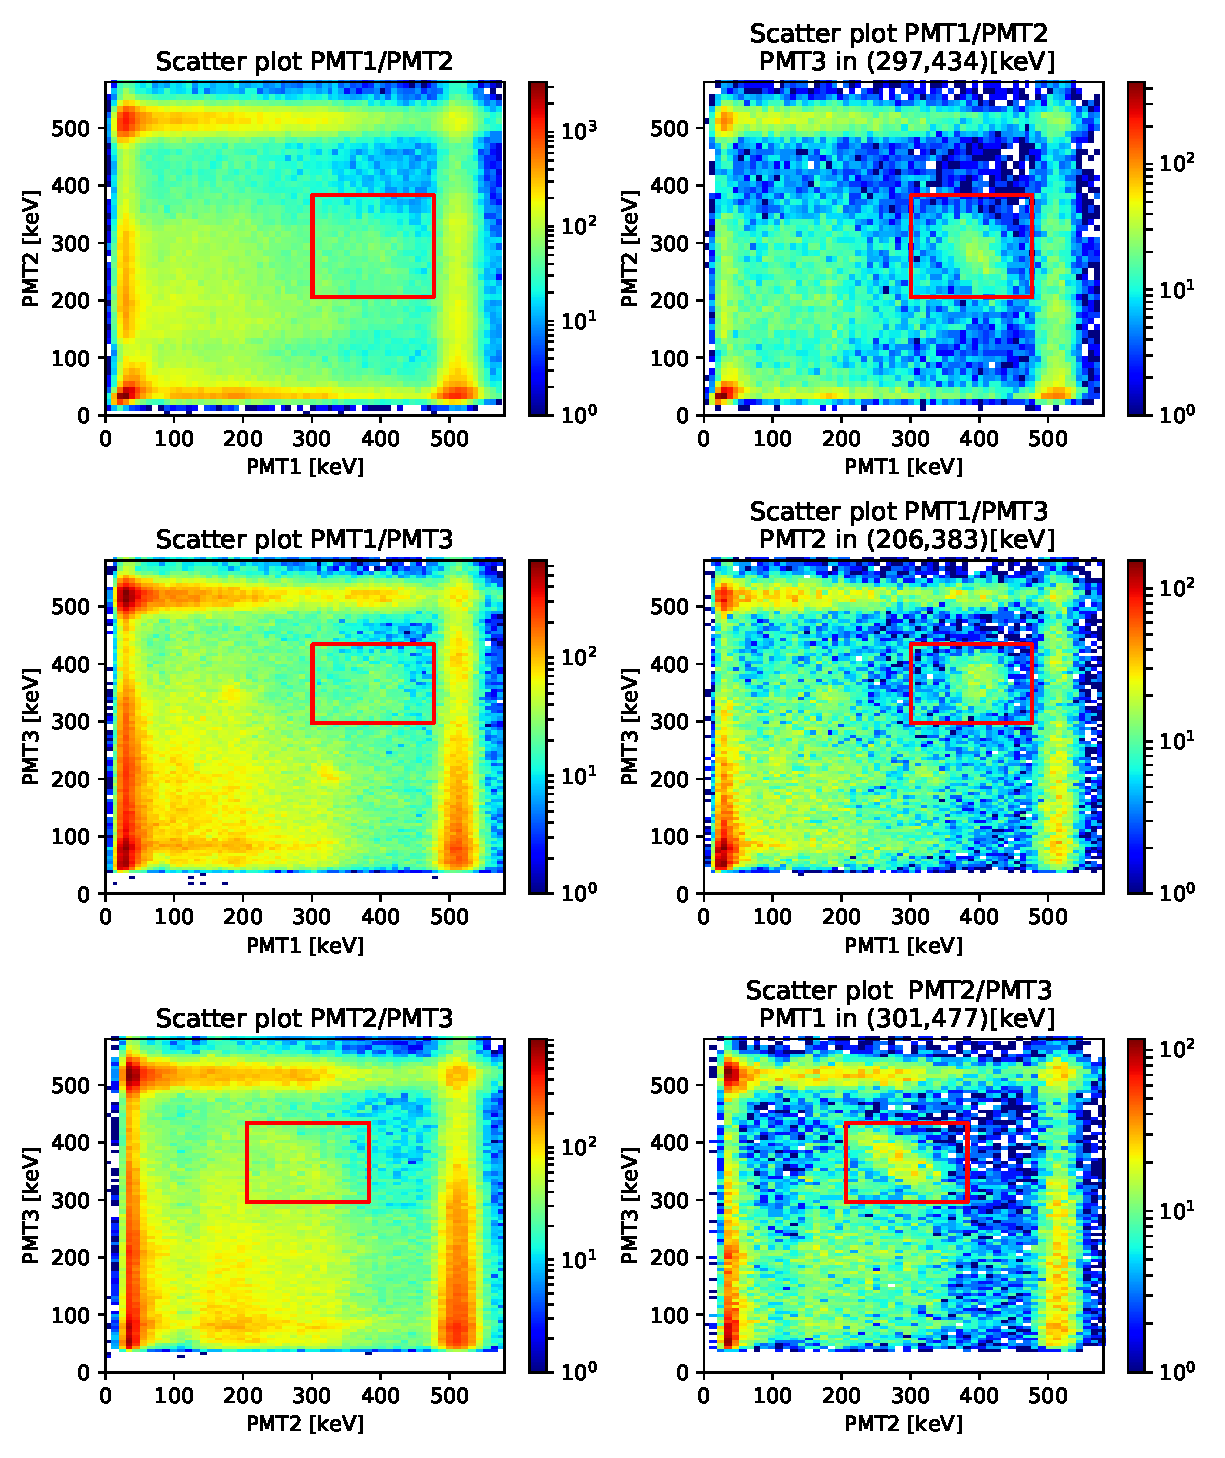
\includegraphics[width=44em]{immagini/3gamma_signal}
	\caption{\label{fig:3gamma_signal} I dati qui rappresentati sono le coincidenze a 3 di una delle 2 prese dati di segnale. Nella colonna di sinistra sono mostrati gli spettri 2D di ciascuna coppia di rivelatori; nella colonna di destra sono mostrati gli spettri 2D di ciascuna coppia di rivelatori dove sono stati selezionati solo gli eventi con energia nell'altro rivelatore in un certo intervallo centrato sul segnale atteso. I box rossi indicano i limiti degli intervalli su ciascun rivelatore. Il segnale è chiaramente visibile nel box.}
\end{figure}

 \begin{figure}[h]
	\hspace{-4em}
	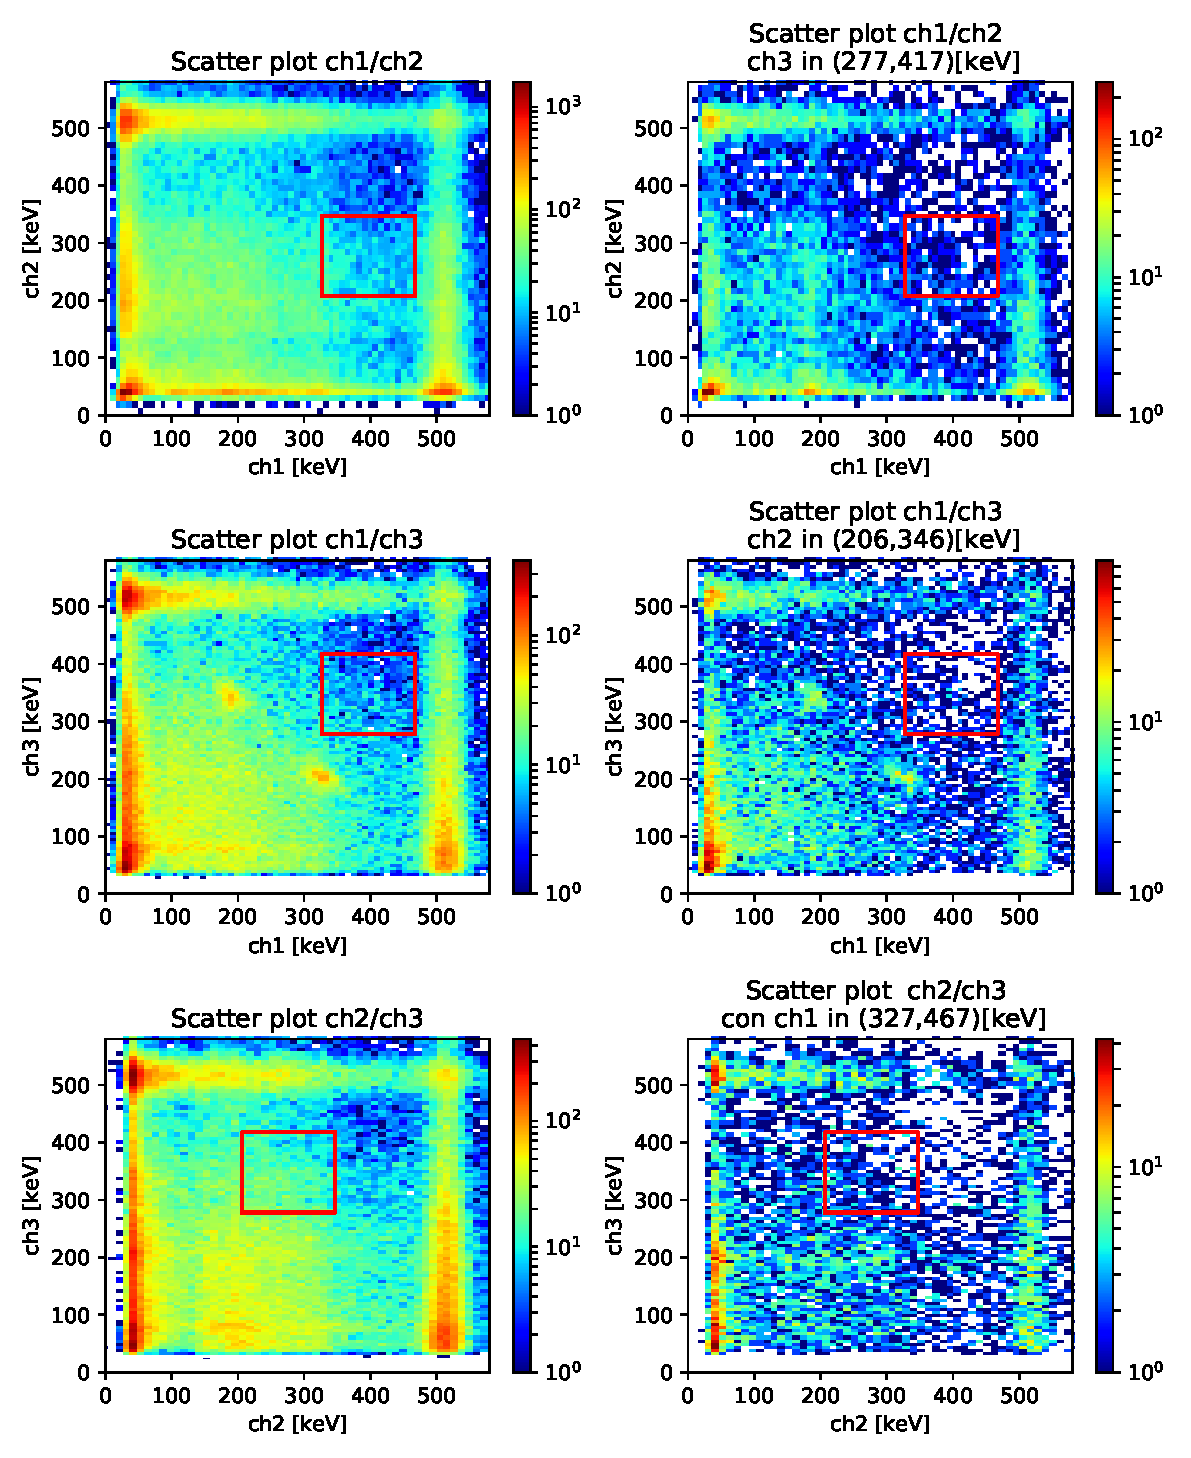
\includegraphics[width=44em]{immagini/3gamma_noise}
	\caption{\label{fig:3gamma_noise} I dati qui rappresentati sono le coincidenze a 3 nella presa dati di rumore. Nella colonna di sinistra sono mostrati gli spettri 2D di ciascuna coppia di rivelatori; nella colonna di destra sono mostrati gli spettri 2D di ciascuna coppia di rivelatori dove sono stati selezionati solo gli eventi con energia nell'altro rivelatore in un certo intervallo centrato sul segnale atteso. I box rossi indicano i limiti degli intervalli su ciascun rivelatore. Nessun segnale è visibile nel box.}
\end{figure}

	

%realizzazione esperimento


%analisi